\documentclass[10pt]{article}
\usepackage[margin=0.65in]{geometry}\usepackage[T1]{fontenc}\usepackage{graphicx}
\begin{document}\section*{Finite private assembly and shared-cost reservation}
The coordinator records USD1 for one bounded existing-host assembly and its storage share, plus USD55 for observed standing resources and delayed spending. The daily reported headroom is USD68.87; reserving USD56 leaves an estimated USD12.87. These are conservative accounting estimates.
\begin{center}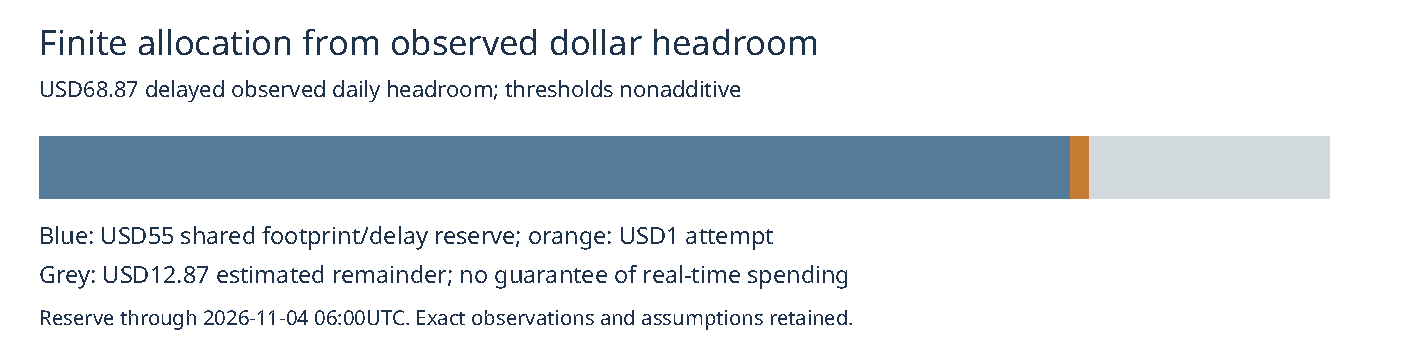
\includegraphics[width=\linewidth]{diagram.pdf}\end{center}
\textbf{Attempt allocation.} The existing m8i.8xlarge Spot request cap is USD1.69344/hour. Charging its entire host for 600 seconds gives USD0.28224. Allocating 4GiB of existing gp3 storage through the deadline adds approximately USD0.005478. No new EC2 or EBS resource is created. The allocation is USD1.

\textbf{Shared footprint.} The retained observations identify three instances, 49gp3 volumes (4666GiB), 60standard snapshots (6794GiB full source-size upper estimate), one EKS cluster and one NAT gateway. Conservative hourly charges total USD3.411890. Over the interval from the delayed budget observation through 06:00UTC, this is USD42.050365; the USD55 reserve includes USD12.949635 extra margin.

\textbf{Assumptions and conditions.} The margin estimates variable or omitted S3, transfer, NAT traffic, IPv4, other-region and delayed charges; these are not assumed absent. No additional paid launch is included. Reconcile any known conflicting commitment before launch. Retention beyond the deadline needs a continued allocation or reviewed disposition, preserving failure evidence.

\textbf{Independent admission.} The final non-author review approves one 600-second private assembly at 2CPU, 2GiB RAM and 4GiB disk. It binds the exact source, allocation and worker ledger. Qualification and scientific execution remain separate. Inputs, command and review must be published before launch; timeout or unresolved cleanup does not permit an automatic retry.

\textbf{Evidence.} cost-review.json and observations.tar.gz preserve exact read-only query receipts, pricing and arithmetic. allocation.json records coordinator reservations; assembly-review.json and assembly-binding.json supply the exact admission. This is a cost reservation, not a scientific comparison.
\end{document}